\documentclass{eh-homework}

\begin{document}
\usetikzlibrary{arrows.meta}
\begin{question}{1}
\textbf{(5.1, \#18)} The Bézier curve
\[
x(t) = 11t^3 - 18t^2 + 3t + 5
\]
\[
y(t) = t^3 + 1
\]
has control points \((5,1)\), \((6,1)\), and \((1,2)\). Find the fourth control point.

\bigskip

Notice that \((x(0), y(0)) = (5,1)\) and \((x(1), y(1)) = (1,2)\), so \((5,1), (1,2)\) are the first and last control points. Let us suppose that \((a,b)\) is the missing control point, and it is ordered second. Then the B\'ezier curve with the control points above should have the form
\begin{align*}
    x(t) &= 5(1-t)^3 + 3at(1-t)^2 + 18t^2(1-t) + t^3 \\
    &= (-5 + 3a - 18 + 1)t^3 + (15 - 6a + 18)t^2 + (-15 + 3a)t + 5 \\
    &= (3a - 22)t^3 + (- 6a + 33)t^2 + (3a - 15)t + 5
\end{align*}
\begin{align*}
    y(t) &= (1-t)^3 + 3bt(1-t)^2 + 3t^2(1-t) + 2t^3 \\
    &= (-1 + 3b - 3 + 2)t^3 + (3 - 6b + 3)t^2 + (-3 + 3b)t + 1 \\
    &= (3b - 2)t^3 + (- 6b + 6)t^2 + (3b - 3)t + 1
\end{align*}
We attempt to equate coefficients of \(x(t)\), and obtain that \(a = 11 = \frac{17}{2}\), which is impossible. Thus it must be true that \((a,b)\) is the third control point in order. We perform similar calculations to get that
\begin{align*}
    x(t) &= 5(1-t)^3 + 18t(1-t)^2 + 3at^2(1-t) + t^3 \\
    &= (-5 + 18 - 3a + 1)t^3 + (15 - 36 + 3a)t^2 + (-15 + 18)t + 5 \\
    &= (-3a + 14)t^3 + (3a - 21)t^2 + 3t + 5
\end{align*}
and
\begin{align*}
    y(t) = (3b - 2)t^3 + (- 6b + 6)t^2 + (3b - 3)t + 1.
\end{align*}
It can be shown that \(a = 1, b = 1\) by equating coefficients. Thus the missing third control point is \((1,1)\).
\end{question}
\newpage
\begin{question}{2}
Sketch a stencil for the following data, picking appropriate \(x_0\) and \(h\), that can be used to approximate \(f'(1)\). You do not need to derive the formula.

\[
\begin{array}{c|cccc}
x & -3 & -1.5 & 0 & 2 \\
\hline
f(x) & 3.11 & 3.05 & 3.4 & 3.7 \\
\end{array}
\]

\bigskip

We let \(x_0 = -3\), \(h = 1\). Then the stencil looks like this:
\begin{center}
    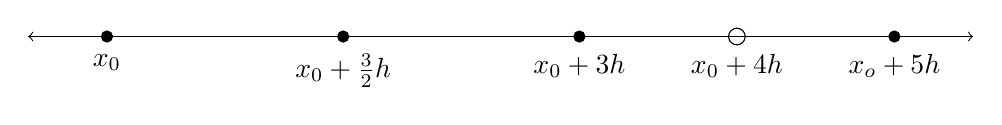
\begin{tikzpicture}
        \draw[<->] (-7, 0) -- (5, 0);
        \foreach \x\val in {-6/\(x_0\), -3/\(x_0 + \frac{3}{2}h\), 0/\(x_0 + 3h\), 4/\(x_o + 5h\)} {
            \draw[fill] (\x, 0) circle (2pt);
            \node[below] at (\x, -0.1) {\val};
        }
        \draw (2, 0) circle (3pt);
        \node[below] at (2, -0.1) {\(x_0 + 4h\)};
    \end{tikzpicture}
\end{center}
\end{question}
\newpage
\begin{question}{3}
\textbf{(4.1, \#13c)} Derive an approximation formula for the second derivative \( f'' \) over the stencil:

\begin{center}
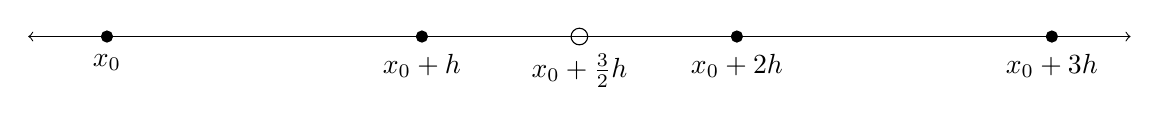
\begin{tikzpicture}
    \draw[<->] (-7,0) -- (7,0) node[below]{};
    \foreach \x/\label in {-6/\(x_0\), -2/\(x_0 + h\), 2/\(x_0 + 2h\), 6/\(x_0 + 3h\)} {
        \draw[fill] (\x, 0) circle (2pt);
        \node[below] at (\x,-0.1) {\label};
    }
    \draw (0, 0) circle (3pt);
    \node[below] at (0, -0.1) {\(x_0 + \frac{3}{2}h\)};
\end{tikzpicture}
\end{center}

using a direct method as discussed in Section 4.1.

\bigskip

We begin by finding the interpolating polynomial of least degree for this stencil. Using Lagrange's interpolation formula:
\[
    L(x_0 + \theta h) = \frac{(\theta - 1)(\theta - 2)(\theta - 3)}{(-1)(-2)(-3)}f(x_0) + \frac{\theta(\theta - 2)(\theta - 3)}{(1)(-1)(-2)}f(x_0 + h)
\]
\[
    + \frac{\theta(\theta - 1)(\theta - 3)}{(2)(1)(-1)}f(x_0 + 2h) + \frac{\theta(\theta - 1)(\theta - 2)}{(3)(2)(1)}f(x_0 + 3h)
\]
\[
    = -\frac{\theta ^3 -6 \theta ^2 + 11 \theta - 6}{6}f(x_0) + \frac{\theta ^3 -5 \theta ^2 + 6 \theta}{2}f(x_0 + h)
\]
\[
    - \frac{\theta ^3 - 4 \theta ^2 + 3 \theta}{2}f(x_0 + 2h) + \frac{\theta ^3 - 3 \theta^2 + 2 \theta}{6}f(x_0 + 3h)
\]
We take the derivative twice with respect to \(\theta\) to get that
\[
    h^2L''(x_0 + \theta h) = -\frac{6\theta - 12}{6}f(x_0)+\frac{6 \theta - 10}{2}f(x_0 + h)-\frac{6\theta - 8}{2}f(x_0 + 2h)+\frac{6\theta - 6}{6}f(x_0 + 3h)
\]
\[
    = (2- \theta)f(x_0) +(3\theta - 5)f(x_0 + h)+(4 - 3\theta)f(x_0 + 2h)+(\theta - 1)f(x_0 + 3h)
\]
Substituting \(\theta = \frac{3}{2}\) gives us the required approximation formula:
\[
    f''\left( x_0 + \frac{3}{2}h \right) \approx \frac{1}{h^2}\left( \frac{1}{2}f(x_0) - \frac{1}{2} f(x_0 + h) - \frac{1}{2} f(x_0 + 2h) + \frac{1}{2}f(x_0 + 3h) \right) 
\]
\end{question}
\newpage
\begin{question}{4}
\textbf{(4.2, \#3c)} Over the same stencil as in the previous question, derive an approximation formula for the second derivative \( f'' \) but now using undetermined coefficients.

\bigskip

Let our formula be of the form
\[
    a_0 f(x_0) + a_1 f(x_0 + h) + a_2 f(x_0 + 2h) + a_3 f(x_0 + 3h).
\]
For \(i = 0, 1, 2, 3\), the formula is exact for functions \(f_i (x) = \left(x - x_0\right)^i\). Thus using each function, we have the system of equations
\begin{align*}
    0 &= a_0 + a_1 + a_2 + a_3 \\
    0 &= h a_1 + 2h a_2 + 3h a_3 \\
    2 &= h^2 a_1 + 4h^2 a_2 + 9h^2 a_3 \\
    9h &= h^3 a_1 + 8 h^3 a_2 + 27 h^3 a_3
\end{align*}
which we can solve by row reducing the matrix
\begin{align*}
    \left( \begin{array}{@{}cccc|c@{}}
        1 & 1 & 1 & 1 & 0 \\
        0 & h & 2h & 3h & 0 \\
        0 & h^2 & 4h^2 & 9h^2 & 2 \\
        0 & h^3 & 8h^3 & 27h^3 & 9h
    \end{array} \right)
    &\rightarrow
    \left( \begin{array}{@{}cccc|c@{}}
        1 & 0 & -1 & -2 & 0 \\
        0 & 1 & 2 & 3 & 0 \\
        0 & 0 & 2h^2 & 6h^2 & 2 \\
        0 & 0 & 6h^2 & 24h^2 & 9
    \end{array} \right)
    \rightarrow
    \left( \begin{array}{@{}cccc|c@{}}
        1 & 0 & -1 & -2 & 0 \\
        0 & 1 & 2 & 3 & 0 \\
        0 & 0 & 2h^2 & 6h^2 & 2 \\
        0 & 0 & 0 & 6h^2 & 3
    \end{array} \right) \\
    &\rightarrow
    \left( \begin{array}{@{}cccc|c@{}}
        1 & 0 & -1 & -2 & 0 \\
        0 & 1 & 2 & 3 & 0 \\
        0 & 0 & 1 & 0 & -\frac{1}{2h^2} \\
        0 & 0 & 0 & 1 & \frac{1}{2h^2}
    \end{array} \right)
    \rightarrow
    \left( \begin{array}{@{}cccc|c@{}}
        1 & 0 & 0 & 0 & \frac{1}{2h^2} \\
        0 & 1 & 0 & 0 & -\frac{1}{2h^2} \\
        0 & 0 & 1 & 0 & -\frac{1}{2h^2} \\
        0 & 0 & 0 & 1 & \frac{1}{2h^2}
    \end{array} \right)
\end{align*}
Therefore our approximating formula for \(f''\left( x_0 + \frac{3}{2}h \right)\) is
\[
    \frac{1}{2h^2}f(x_0) - \frac{1}{2h^2}f(x_0 + h) - \frac{1}{2h^2}f(x_0 + 2h) + \frac{1}{2h^2}f(x_0 + 3h)
\]
which is consistent with the formula we obtained in the previous question.
\end{question}
\newpage
\begin{question}{5}
\textbf{(Based on 4.1, \#19)} Let \( x_0, x_0 + \alpha h, x_0 + 2h \) be nodes where \( \alpha \neq 0,2 \).

\begin{enumerate}[label=\alph*.]
    \item Write the first Taylor polynomials of \( f(x_0 +\alpha h) \) and \( f(x_0 +2h) \) around \( x = x_0 \), then use these to show that:
    \[
    f'(x_0) = \frac{1}{2h} \left[ -\frac{2+\alpha}{\alpha} f(x_0) + \frac{4}{\alpha(2-\alpha)} f(x_0 + \alpha h) - \frac{\alpha}{2-\alpha} f(x_0 + 2h) \right].
    \]

    Assuming \(f\) is analytic, the Taylor series expansion of \(f\) around \(x = x_0\) is
    \[
        f(x) = \sum_{n=0}^{\infty} \frac{f^{(n)}(x_0)}{n!}(x - x_0)^n
    \]
    so
    \[
        f(x_0 + \alpha h) \approx f(x_0) + f'(x_0) \alpha h \text{ and } f(x_0 + 2h) \approx f(x_0) + f'(x_0) 2h.
    \]
    We see that
    \begin{align*}
        &\ \frac{1}{2h} \left[ -\frac{2+\alpha}{\alpha} f(x_0) + \frac{4}{\alpha(2-\alpha)} f(x_0 + \alpha h) - \frac{\alpha}{2-\alpha} f(x_0 + 2h) \right] \\
        &= \frac{1}{2h} \left[ -\frac{2+\alpha}{\alpha} f(x_0) + \frac{4}{\alpha(2-\alpha)} (f(x_0) + f'(x_0) \alpha h) - \frac{\alpha}{2-\alpha} (f(x_0) + f'(x_0) 2h) \right] \\
        &= \frac{1}{2h}\left[ \left( -\frac{2}{\alpha} - 1 + \frac{4}{\alpha (2 - \alpha)} - \frac{\alpha}{2 - \alpha} \right) f(x_0) + \left( \frac{4h}{2 - \alpha} - \frac{2\alpha h}{2 - \alpha} \right) f'(x_0) \right] \\
        &= \frac{1}{2h}\left[ \left( -\frac{2}{\alpha} - 1 + \frac{2}{\alpha} + \frac{2}{2 - \alpha} + 1 - \frac{2}{2 - \alpha} \right) f(x_0) + \frac{2h(2 - \alpha)}{2 - \alpha} f'(x_0) \right] \\
        &= \frac{1}{2h}[2h f'(x_0)] \\
        &= f'(x_0)
    \end{align*}
    as needed.

    \item Now show that the same result is obtained when using the method of undetermined coefficients.
    
    Let
    \[
        f'(x_0) \approx a_0 f(x_0) + a_1 f(x_0 + \alpha h) + a_2 f(x_0 + 2h).
    \]
    Choose functions \(f_i(x) = (x - x_0)^i\), for \(i = 0,1,2\). It follows that
    \begin{align*}
        0 &= a_0 + a_1 + a_2 \\
        1 &= \alpha h a_1 + 2h a_2 \\
        0 &= \alpha ^2 h^2 a_1 + 4h^2 a_2
    \end{align*}
    We solve by row reducing, keeping in mind that we never perform division by 0 since \(\alpha \neq 0,2\):
    \begin{align*}
        \left( \begin{array}{@{}ccc|c@{}}
            1 & 1 & 1 &  0 \\
            0 & \alpha h & 2h &  1 \\
            0 & \alpha^2 h^2 & 4h^2 &  0 \\
        \end{array} \right)
        &\rightarrow
        \left( \begin{array}{@{}ccc|c@{}}
            1 & 1 & 1 &  0 \\
            0 & \alpha^2 h^2 & 4h^2 &  0 \\
            0 & 0 & 2h - \frac{4h}{\alpha} &  1 \\
        \end{array} \right)
        \rightarrow
        \left( \begin{array}{@{}ccc|c@{}}
            1 & 0 & 1 - \frac{4}{\alpha^2} &  0 \\
            0 & 1 & \frac{4}{\alpha^2} &  0 \\
            0 & 0 & 2h - \frac{4h}{\alpha} &  1 \\
        \end{array} \right) \\
        &\rightarrow
        \left( \begin{array}{@{}ccc|c@{}}
            1 & 0 & 1 - \frac{4}{\alpha^2} &  0 \\
            0 & 1 & \frac{4}{\alpha^2} &  0 \\
            0 & 0 & 1 &  \frac{\alpha}{2h(\alpha - 2)} \\
        \end{array} \right)
        \rightarrow
        \left( \begin{array}{@{}ccc|c@{}}
            1 & 0 & 0 &  -\frac{2 + a}{2\alpha h} \\
            0 & 1 & 0 &  - \frac{2}{\alpha h(\alpha -2)} \\
            0 & 0 & 1 &  \frac{\alpha}{2h(\alpha - 2)} \\
        \end{array} \right)
    \end{align*}
    Thus \(a_0 = -\frac{2 + a}{2\alpha h}, a_1 = - \frac{2}{\alpha h(\alpha -2)}, a_2 = \frac{\alpha}{2h(\alpha - 2)}\), so
    \[
        f'(x_0) \approx \frac{1}{2h}\left[ -\frac{2+\alpha}{\alpha}f(x_0) + \frac{4}{\alpha (2 - \alpha)}f(x_0 + \alpha h) - \frac{\alpha}{2-\alpha}f(x_0 + 2h)\right] 
    \]
    as expected.
\end{enumerate}
\end{question}
\newpage
\begin{question}{6}
\textbf{(4.2, \#4i)} Use undetermined coefficients to derive an approximation formula for the integral over the stencil:

\begin{center}
\begin{tikzpicture}
    \draw[<->] (-1,0) -- (7,0);
    \draw[{Bracket[width=3mm]}-{Bracket[width=3mm]}] (0, 0) -- (6,0);
    \foreach \x/\label in {0/\(x_0\), 4/\(x_0 + \frac{4}{3}h\), 6/\(x_0 + 2h\)} {
        \draw[fill] (\x, 0) circle (2pt);
        \node[below] at (\x,-0.1) {\label};
    }

\end{tikzpicture}
\end{center}

Suppose that
\[
    \int _{x_0}^{x_0 + 2h} f \approx a_0 f(x_0) + a_1 f \left( x_0 + \frac{4}{3}h \right) + a_2 f(x_0 + 2h).
\]
This is exact when \(f\) is a polynomial of degree 2 or less. Pick \(f_i(x) = (x - x_0)^i\), for \(i = 0,1,2\). Then
\begin{align*}
    2h &= a_0 + a_1 + a_2 \\
    2h^2 &= \frac{4}{3}h a_1 + 2h a_2 \\
    \frac{8}{3}h^3 &= \frac{16}{9}h^2 a_1 + 4h^2 a_2
\end{align*}
\begin{align*}
    2h &= a_0 + a_1 + a_2 \\
    \implies h &= \frac{2}{3} a_1 + a_2 \\
    \frac{2}{3}h &= \frac{4}{9} a_1 + a_2
\end{align*}
We solve this system:
\begin{align*}
    \left( \begin{array}{@{}ccc|c@{}}
        1 & 1 & 1 & 2h \\
        0 & \frac{2}{3} & 1 & h \\
        0 & \frac{4}{9} & 1 & \frac{2h}{3}
    \end{array} \right) 
    &\rightarrow
    \left( \begin{array}{@{}ccc|c@{}}
        1 & 0 & -\frac{1}{2} & \frac{h}{2} \\
        0 & 1 & \frac{3}{2} & \frac{3h}{2} \\
        0 & 0 & \frac{1}{3} & 0
    \end{array} \right)
    \rightarrow
    \left( \begin{array}{@{}ccc|c@{}}
        1 & 0 & 0 & \frac{h}{2} \\
        0 & 1 & 0 & \frac{3h}{2} \\
        0 & 0 & 1 & 0
    \end{array} \right)
\end{align*}
Thus \(a_0 = \frac{h}{2}, a_1 = \frac{3h}{2}, a_2 = 0\) so our formula is
\[
    \int _{x_0}^{x_0 + 2h} f \approx \frac{h}{2}\left( f(x_0) + 3f \left( x_0 + \frac{4h}{3} \right) \right) 
\]
\end{question}
\end{document}